% !TEX encoding = UTF-8 Unicode

\documentclass[a4paper]{article}

\usepackage{color}
\usepackage{url}
\usepackage[T2A]{fontenc} 
\usepackage[utf8]{inputenc}
\usepackage{graphicx}

\usepackage[english,serbian]{babel}
\usepackage[unicode]{hyperref}
\hypersetup{colorlinks,citecolor=green,filecolor=green,linkcolor=blue,urlcolor=blue}

\begin{document}

\title{Digitalni blizanac\\ \small{Seminarski rad u okviru kursa\\Računarstvo i društvo\\ Matematički fakultet}}

\author{Marko Bura\\ mi18141@alas.matf.bg.ac.rs}
\date{10.~maj 2022.}
\maketitle

\abstract{
Ovaj rad se bavi tehnologijom Digitalni blizanac. Obrađuje osnovne koncepte tehnologije, uvodi čitaoca u tehnologiju kroz terminologiju i izazove sa kojima se susretao i sa kojima se susreće Digitalni blizanac. Takođe govori o širokim primenama ove tehnologije, fokus je i na socijalno-ekonomskom uticaju Digitalnog blizanca i kako ga čovečanstvo doživljava.
\tableofcontents

\newpage

\section{Uvod, poreklo i razvoj sajber-fizičkih softvera}
\label{sec:uvod}

Sa razvojem veštačke inteligencije, pametne tehnologije poput Internet stvari (eng.~{\em Internet of Things - IoT}) , Računarstva u oblaku (eng. ~{\em Cloud Computing - CC}), Analitike velikih podataka (eng. ~{\em Big Data Analytics - BDA}), Sajber-fizičkih sistema (eng. ~{\em Cyber–Physical Systems - CPS}), Digitalnih blizanaca (eng. ~{\em Digital Twin - DTs}) zauzimaju centralnu poziciju u novoj generaciji inteligentnih načina
proizvodnje (eng. ~{\em intelligent manufacturing}). \cite{digitaltwins} 

\begin{figure}[h!]
	\begin{center}
		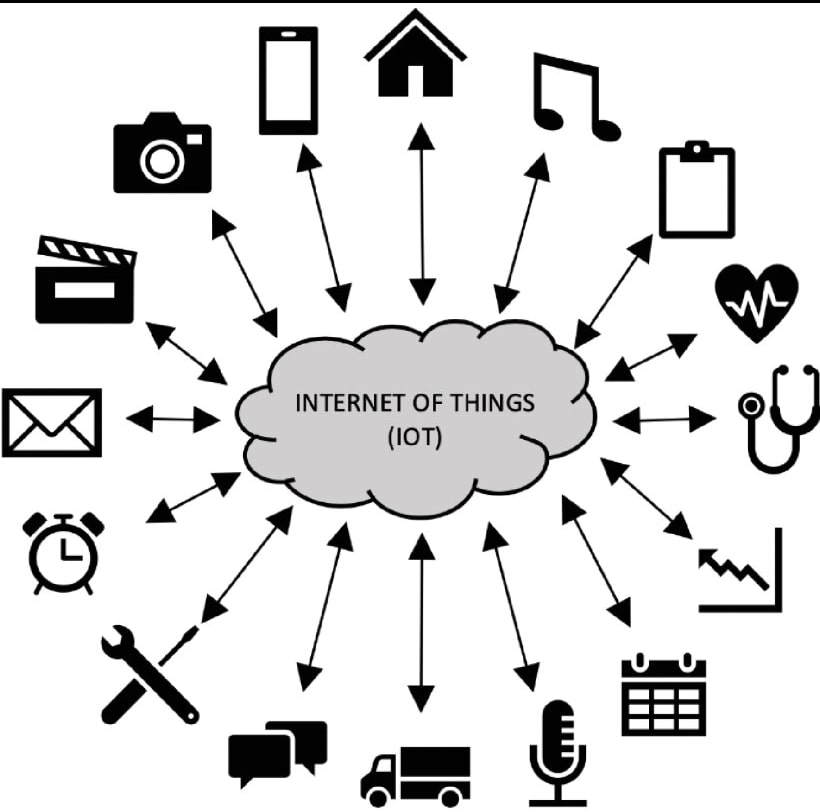
\includegraphics[scale=0.2]{1_internet_of_things.jpg}
	\end{center}
	\caption{IoT dijagram \cite{enablingtechnologies}}
\end{figure}

Proizvodnja sada prelazi sa one bazirane isključivo na znanju na onu čija je osnova u suštini
pametno kreiranje i upotreba podataka u cilju proširivanja znanja. Napredne informacije,
tehnologije za komunikaciju kao i različite analize podataka upravo tome i doprinose.\cite{digitaltwins}

Integracija sajber i fizičkog je zapravo preteča ovakve vrste proizvodnje i predstavlja njenu
suštinu. Upravo je to proslavilo CPS i DT što je dovelo do povećanja popularnosti od strane
akademije, industrije, vlade.\cite{digitaltwins}

CPS su multidimenzionalni i kompleksni sistemi koji vrše integraciju sajber i dinamičkog
fizičkog sveta. Kroz kolaboraciju i spajanje računarstva (eng. ~{\em computing}), kontrole (eng. ~{\em control}) i komunikacije (eng. ~{\em communication}) poznatije i kao
3C, ovi sistemi obezbeđuju povratne informacije, dinamičku kontrolu kao i druge usluge u
trenutnom vremenu. To uslovljava veliku međuzavisnost i povezanost ova dva sveta.\cite{digitaltwins}

CPS predstavlja širok rang aplikacija u različitim sektorima, uključujući proizvodnju, energetiku,
zdravstvo, nadgledanje ključnih infrastruktura kao i potrošačke usluge. Oni predstavljaju
kompleksne, fleksibilne i adaptivne sisteme čiji su elementi okarakterisani povećanom
autonomijom i inteligencijom.\cite{cyber}

\newpage

Samo neke od definicija digitalnog blizanca su:
\begin{itemize}
\item CHEN (2017): Digitalni blizanac je kompjuterizovan model fizičkih uređaja ili sistema koji reprezentuje sve funkcionalnosti i veze sa radnim elementima.\cite{enablingtechnologies}
\item LIU (2018): Digitalni blizanac je živi model fizičkog sredstva i sistema koji se stalno prilagođava operativnim promenama na osnovu prikupljenih online podataka i
informacija i može predvideti budućnost odgovarajućeg fizičkog predstavnika.\cite{enablingtechnologies}
\item ZHENG (2018): Digitalni blizanac predstavlja set virtuelnih informacija koji u potpunosti opisuje potencijalnu ili stvarnu fizičku proizvodnju sa mikro-atomskog nivoa na makro-geometrijski nivo.\cite{enablingtechnologies}
\end{itemize} 

\begin{figure}[h!]
	\begin{center}
		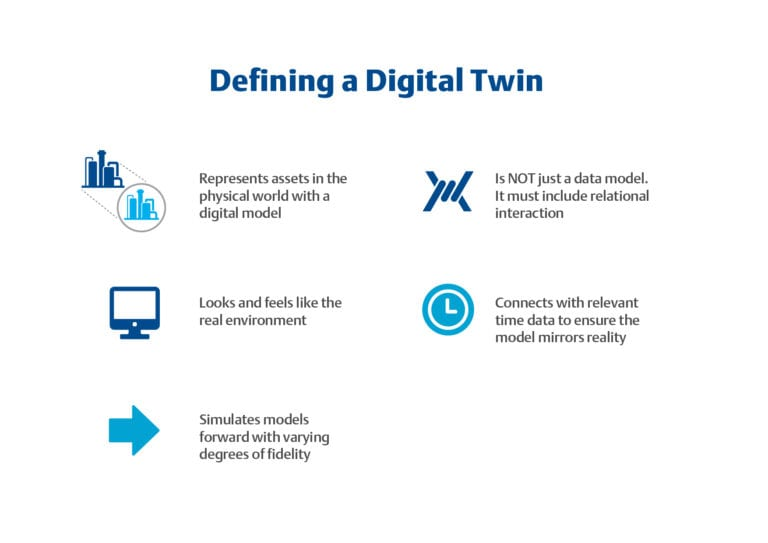
\includegraphics[scale=0.33]{2_definition_of_digital_twin.jpg}
	\end{center}
	\caption{Definisanje Digitalnog blizanca \cite{understanding}}
\end{figure}

DT kreiraju visoko pouzdane virtuelne modele fizičkih objekata u virtuelnom prostoru u cilju da
simuliraju njihova ponašanja u stvarnom svetu i obezbede povratnu informaciju. Zbog potpune
digitalizacije proizvoda, kompanije su u mogućnosti da na vreme pouzdano predvide i lociraju
bilo kakve probleme u proizvodnji, da optimizuju sam proces proizvodnje i da kao rezultat
dobiju što bolje proizvode.\cite{enablingtechnologies}

Glavna namena DT je da se ponaša kao jedini izvor informacija za svog predstavnika iz realnog
sveta. Povezuje različite sisteme na nivou proizvoda i koristi se da struktuira, nadgleda i
upotrebljava podatke. Ono što daje na značaju ovoj tehnologiji je upravo povezivanje
informacija mnogih funkcionalnosti i sistema da unapređuju jedna drugu u realnom vremenu i na
taj način pruže informacije korisniku sa jedne pristupne tačke.\cite{digitaltwins}

Integrisanje fizičkih procesa i kompjuterskih sistema je glavni izazov. Kompjuterski (sajber) deo
konstantno mora da nadgleda stanje fizičkog sistema i u skladu sa tim da primenjuje odluke i
akcije kako bi sproveo kontrolu.\cite{cyber}

\begin{figure}[h!]
	\begin{center}
		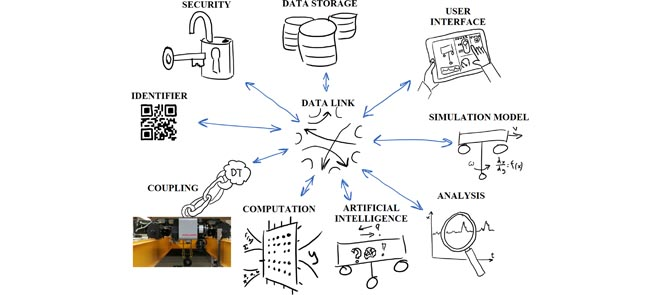
\includegraphics[scale=1.4]{3_access-gagraphic.jpg}
	\end{center}
	\caption{Konceptualni ideal okvira digitalnog blizanca
	zasnovanog na karakteristikama \cite{feature}}
\end{figure}

\section{Terminologija}
\label{sec:terminologija}

\textbf{Digitalni blizanac} (eng. ~{\em Digital Twin - DT}) je virtuelni entitet koji je povezan sa entitetom realnog sveta. On opisuje
planirani ili realni objekat sa najboljom mogućom preciznošću. Informacije mogu biti
distribuirane putem različitih sistema, dok se delovi informacija mogu povezati jedna sa drugom
stvarajući jedan koherentan entitet. \cite{feature}\\

\textbf{Instanca digitalnog blizanca} (eng. ~{\em Digital Twin Instance - DTI}) definiše se kao jedan virtuelni predstavnik jednog određenog
objekta iz realnog sveta. Taj objekat može biti fizički proizvod, čovek, grad, proces ili čak i
događaj, bilo šta što može imati koristi od predstavljanja u virtuelnom svetu. Kako je DTI jedan
interfejs za podatke realnog objekta on mora biti sve vreme prisutan na Internetu kako bi
obezbedio konstantan protok podataka. Svaki DTI ima jedinstven identifikator koji se koristi za
konektovanje iz bilo kog dela sveta.\cite{feature}\\
 
\textbf{Blok Digitalnog blizanca} (eng. {\em Digital Twin Block - DTB}) je podsistem DTI. Predstavlja nezavisan softverski entitet koji može
biti konektovan na drugi DTB kako bi oformio DTI.\cite{feature}\\

\textbf{Klasa Digitalni blizanac} (eng. ~{\em Digital Twin Class - DTC}) je alat za kreiranje DTI, na sličan način kao što objektno-orijentisani
programski jezici koriste klase kao alate da bi kreirali instance objekata. Akcenat se stavlja na
kreiranje DTI.\cite{feature}\\

\textbf{Funkcionalnost Digitalnog blizanca} (eng. ~{\em Digital Twin Feature - DTF}) je zajednički termin za različite vrste tehničkih funkcionalnosti
DT. To je dodatni sloj apstrakcije koji obezbeđuje tranziciju od funkcionalnih zahteva do
tehničke implementacije.\cite{feature}\\


Izdvajaju se sledeće analize bazirane na ovim funkcionalnostima:
\begin{itemize}
\item \textbf{Utemeljena teorija} (eng. ~{\em Grounded theory}): Osnovna ideja metodologije je da proizvede teorije koje su zasnovane na
podacima. Osnovni elementi uključuju kategorizaciju podataka, pronalaženje relacija između
kategorija i konačno integrisanje kategorija s ciljem razvijanja teorije. Ova teorija zahteva
simultano prikupljanje podataka, analizu i razvijanje teorije od trenutka započinjanja procesa
istraživanja. Razvijanje teorije je inicirano kategorizacijom podataka, što je dovelo do
prepoznavanja DTF. \cite{feature}

\begin{figure}[h!]
	\begin{center}
		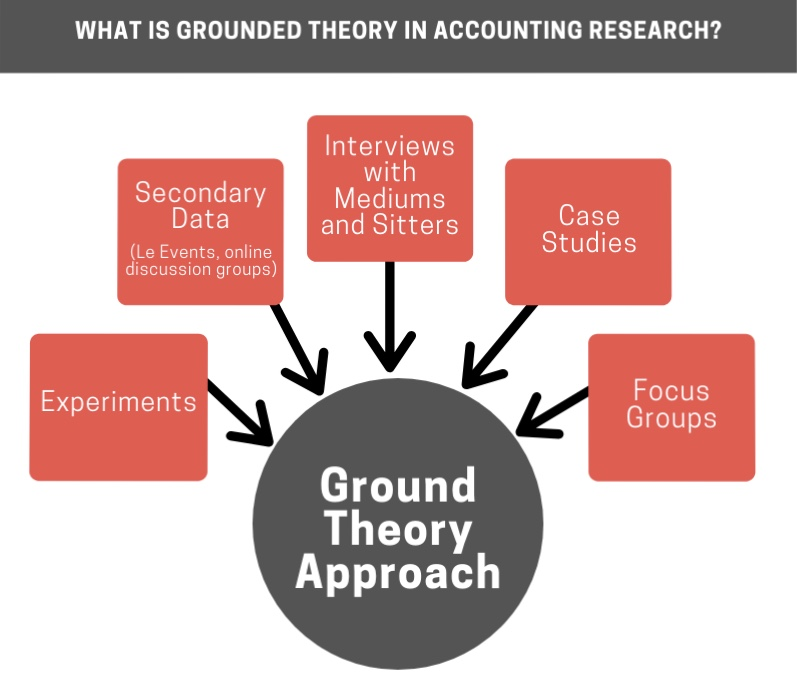
\includegraphics[scale=0.33]{4_grounded_theory.jpg}
	\end{center}
	\caption{Pristup na kome se zasniva utemeljena teorija\cite{groundedteory}}
\end{figure}

\item \textbf{Korelaciona analiza}: Korelacija predstavlja normalizovanu linearnu sličnost između dva faktora.
Normalizacija povezuje maksimalnu vrednost sa 1 a minimalnu sa -1. Vrednost 1 predstavlja
strogu pozitivnu vezu, ukoliko je jedan faktor ima visoku vrednost imaće i drugi. Ako je
korelacija strogo negativna onda je veza inverzna. Međutim iako su dva faktora u korelaciji to ne
mora značiti da će veza biti kauzalna. Da bi se dokazala kauzalnost veze potrebno je sprovesti
izolovane testove, dokazati zavisnosti pomoću zakona fizike itd. Ova analiza se koristi kao alat
za razumevanje relacija i hijerarhije između DTF. \cite{feature}
\end{itemize}

\section{Koncepti tehnologije Digitalni blizanac}	
\label{sec:koncepti}

Neke od bitnih karakteristika Digitalnog blizanca su: konektivnost, homogenizacija, mogućnost
ponovnog programiranja, digitalni tragovi i modularnost.\\

\textbf{1. Konektivnost:} Tehnologija omogućava povezivanje fizičke komponente i njenog digitalnog
predstavnika. Upravo je osnova DT zasnovana na ovoj vezi, jer bez nje ne bi ni
postojala. Na taj način omogućava povezanost između organizacija, proizvoda i kupaca. \cite{smartconnecting} \\

\textbf{2. Homogenizacija:} Predstavlja razdvajanje fizičkog od digitalnog aspekta DT, iako
se u poslednje vreme sve više informacija o fizičkim proizvodima čuva digitalno i odvaja od
samog proizvoda. Homogenizacija takođe za posledicu razdvajanja informacija ima i
konvergiranje korisničkog iskustva. Kako se informacije sa fizičkih objekata digitalizuju, jedan
objekat može imati višestruke nove mogućnosti. \cite{digitalinfrastructures} \\

\textbf{3. Mogućnost ponovnog programiranja i pametni aspekt:} Postoji mogućnost ponovnog
programiranja odnosno izmene trenutne verzije koda pomoću senzora, na automatski način. Kroz
senzore na fizičkom proizvodu i AI tehnologije, javlja se posledica reprogramabilne prirode. Npr.
kada je u pitanju motor, DT se može koristiti da se prikupe podaci o performansama
motora ili o prilagođavanju i evenutalnom ažuriranju motora.\cite{seeingdouble}\\

\textbf{4. Digitalni tragovi: } U pitanju je neka vrsta tragova koje koriste inženjeri npr. prilikom kvara
mašine kako bi uočili problem i sanirali posledice. Takođe, ove tragove mogu koristiti i u
budućnosti kako bi se javljalo što manje grešaka i kako bi svaka naredna verzija DT
bila što bolja. \cite{sensordata}\\

\textbf{5. Modularnost:} U proizvodnoj industriji se podrazumeva pod dizajn i prilagođavanje proizvoda
i proizvodnih modula. Time se dobija mogućnost podešavanja modela i mašina. Tehnologija
Digitalni blizanac omogućava proizvođačima da prate mašine koje se koriste i uoče moguća područja
poboljšanja u mašinama.\cite{autonomy}

\begin{figure}[h!]
	\begin{center}
		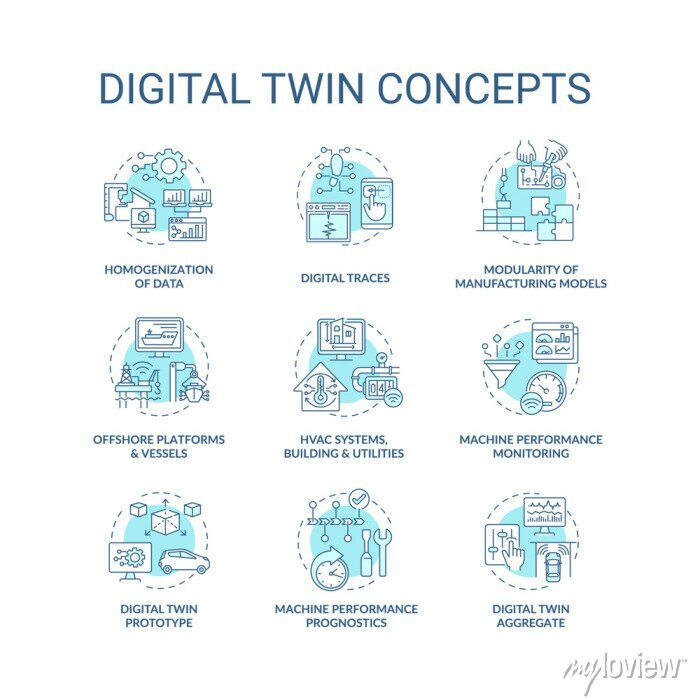
\includegraphics[scale=0.33]{5_concept.jpg}
	\end{center}
	\caption{Koncepti na kojima se zasniva DT\cite{sticker}}
\end{figure}

\section{Izazovi}
\label{izazovi}

Postaje očiglednije da DT radi paralelno sa tehnologijama veštačke inteligencije (AI) i
informacionim tehnologijama (IT) što rezultira zajedničkim izazovima.

Prvi korak u suočavanju sa izazovima je njhovo identifikovanje. Neki od zajedničkih izazova se
mogu pronaći u analizi podataka i IoT, a krajnji cilj je identifikovati zajedničke izazove za
DT. \cite{enablingtechnologies}

Izazovi pri analizi podataka:
\begin{itemize}
\item \textbf{IT infrastruktura:} Izazov u ovoj oblasti je sveden na visoku cenu instalacije i pokretanje
sistema softvera i hardvera. Na primer, troškovi grafičke procesorske jedinice (GPU) visokih
performansi mogu koštati i do nekoliko hiljada dolara. Prevazilaženje ovog izazova možemo
ostvariti pomoću upotrebe GPU-a kao servisa usluge obezbeđivanja procesorske jedinice na
zahtev pomoću tehnologije računarstvo u oblaku. Npr. Amazon, Google i Microsoft pružaju ovakve usluge. \cite{enablingtechnologies}
\item \textbf{Podaci:} bitno je obezbediti da podaci nisu lošeg kvaliteta, moraju biti sortirani i pouzdani.\cite{enablingtechnologies}
\item \textbf{Privatnost i bezbednost:} Propis je jedan korak koji se može preduzeti da bi se osiguralo da su
privatni podaci zaštićeni, dok je drugi metod udruženo učenje. Ono omogućava korisnicima
podataka da ostanu lokalizovani bez ikakvog deljenja podataka, otkrivanja privatnosti i problema
sa bezbednošću pri analizi podataka korišćenjem DT tehnologije.\cite{enablingtechnologies}
\item \textbf{Poverenje:} S obzirom na to da je veštačka inteligencija poprilično nova tehnologija i da je i
dalje u razvoju, postoji opravdana sumnja u njeno funkcionisanje kao i strah da će postati
dominantna u današnjem društvu i na taj način zameniti ljudski uticaj. U medijima su uglavnom
bili prikazani samo negativni uticaji primene ove tehnologije što je dovelo do smanjenog
poverenja kod ljudi. \cite{enablingtechnologies}
\item \textbf{Očekivanja:} Problem je preveliko oslanjanje na veštačku inteligenciju i njenu primenu u
svakodnevnim problemima. Tehnologija je i dalje u razvoju i ne može se očekivati da trenutno
uštedi novac i vreme njenim korisnicima i to treba imati u vidu prilikom njene primene.\cite{enablingtechnologies}
\end{itemize}
Izazovi u oblasti IoT i u IoT industriji:
\begin{itemize}
\item \textbf{Podaci, privatnost, bezbednost i poverenje:} Kako je došlo do velikog rasta u upotrebi IoT
uređaja bilo u kućnoj ili industrijskoj upotrebi, pojavili su se izazovi prilikom prikupljanja velike
količine podataka. Problem nastaje u kontrolisanju protoka podataka i potrebno je obezbediti da
oni budu organizovani i efikasno iskorišćeni. U IoT-u potrebno je upravljati velikom količinom
podataka, voditi računa da oni budu sortirani i organizovani, što će rezultirati time da veća
količina podataka bude iskoristiva i da ima neku vrednost.\cite{enablingtechnologies}
\item \textbf{Infrastruktura:} Unapređivanje stare infrastrukture i integracija sa novim tehnologijama
pomaže u rastu IoT-a. Tako unapređena infrastruktura obezbeđuje mogućnost da se iskoriste
pogodnosti poslednjih tehnologija i snaga aplikacija i servisa dostupnih na oblaku bez potrebe
za obnavljanjem postojećih sistema. Još jedan od izazova u pogledu infrastrukture je povezivanje
starih uređaja sa novim IoT okruženjem, što se moze rešiti njihovim prilagođavanjem novijim
tehnologijama.\cite{enablingtechnologies}
\item \textbf{Povezanost:} Ovaj izazov najčešće nastaje pri nadgledanju sistema u realnom vremenu. Izazovi
obično imaju veze sa pokušajem da se konektuje više korisnika istovremeno. Jedan senzor koji
nije u potpunosti povezan može drastično da utiče na to da krajnji cilj procesa ne bude ostvaren.
Prilagođavanje starijih tehnologija novim je način da se obezbedi da će svi podaci biti
prikupljeni. \cite{enablingtechnologies}
\item \textbf{Očekivanja:} Ovaj izazov odnosi se na to da krajnji korisnici ne razumeju u potpunosti šta da
očekuju od IoT rešenja i kako da ih koriste na najbolji mogući način. Upotreba ove tehnologije
nije moguća bez osnovnog poznavanja tehnologije. Treba obezbediti da se IoT tehnologija
koristi na najbolji način, kako bi se iskoristio njen pun potencijal. \cite{enablingtechnologies}
\end{itemize}

Izazovi kod tehnologije Digitalni blizanac:\\ Neki od izazova se ponavljaju u prethodno navedenim slučajevima kao što su: IT infrastruktura,
privatnost i bezbednost, poverenje i očekivanja.\\
Postoje i novi izazovi svojstveni samo ovoj tehnologiji, a to su:
\begin{itemize}
\item \textbf{Upotrebljivost podataka:} Konstantan protok podataka bez prekida je neophodan jer u
suprotnom može doći do rizika da podaci budu oštećeni ili da neki od podataka nedostaje. \cite{enablingtechnologies}
\item \textbf{Standardizovano modelovanje:} Od samog početka dizajniranja pa sve do simulacije DT mora postojati standardizovan pristup modelovanju. Ovakav pristup obezbeđuje protok
informacija između svake od faza razvoja i implementacije DT. \cite{enablingtechnologies}
\end{itemize}

\section{Tehnologija u upotrebi i primena}
\label{sec:upotreba}
\noindent

\textbf{D9 aplikacioni domen} (eng. ~{\em D9 Application Domain}) se sastoji od tri bitna sloja, prvi sloj je za kreiranje visoko pouzdanih
modela fizičkog entiteta. Vizuelizacija i modelovanje su omoguceni pomoću alata poput
Simulinka-a i Twin Builder-a. Drugi sloj se specifično koristi kao podrška trećem sloju.
Poslednji sloj ovog domena se koristi da bi obezbedio pravilno prikupljanje podataka, a to rade
sledeće aplikacije: Predix, Mindsphere i Storm. \cite{enablingtechnologies}\\

\textbf{D10 domen srednjeg sloja} (eng. ~{\em D10 Middleware Domain}) se sastoji od dva sloja. Prvi sloj omogućava skladištenje podataka
pomoću MongoDB i MySQL servisa i baza podataka koje su neophodne za korišćenje DT. Drugi sloj je u vezi sa procesuiranjem podataka i ključan je za transfer uskladištenih
podataka između D10 i D11 domena. \cite{enablingtechnologies}\\

\textbf{D11 Internet domen} (eng. ~{\em D11 Networking Domain}) ima dva sloja, prvi je neophodan za obezbeđivanje da prikupljeni podaci
komuniciraju između domena. Drugi sloj predstavlja bežični komunikacioni sloj koji je
potreban za obezbeđivanje bežičnog protoka podataka sa odgovarajućim protokolom kao i da
prenese podatke do sledećeg domena. \cite{enablingtechnologies}\\

\textbf{D12 objektni domen} (eng. ~{\em D12 Object Domain}) takođe ima dva sloja koja su neophodna da obezbede pravi hardver koji
će sprovesti analizu Digitalnog blizanca. \cite{enablingtechnologies}

\section{Socijalno-ekonomski uticaj}
\label{sec:socijalni_uticaj}

DT će doneti automatizaciju bez izuzetka u upravljanju bilo kojom fizičkom
imovinom. Jedan od prvih izazova koji može predstavljati prepreku u adaptaciji DT
kao i svih drugih tehnologija automatizacije jeste njegovo prihvatanje od strane zaposlenih.
Strah od gubitka posla izgledao je vrlo logično nekoliko decenija ranije, međutim čak i u to
vreme postojala su i suprotna mišljenja zasnovana na istraživanjima.\cite{values}

Takve studije se fokusiraju na osetljivost radne snage sa nižim kvalifikacijama koja je
uključena u rutinske poslove. Postoje i pozitivni aspekti vezani za automatizaciju koji se mogu
istaći pažljivom raspodelom zadataka između ljudi i mašina. Tako se može omogućiti veća
sigurnost i kreativnost na radnom mestu oslobađanjem dosadnog i sirovog posla koji će
preuzeti mašine i veštačka inteligencija. \cite{values}

Ljudi bi trebalo da, osim koordinisanja razvoja veštačke inteligencije, vode računa i o proveri
rezultata koji se na nju odnose. Pored nekoliko negativnih uticaja Digitalnog blizanca na socijalno-ekonomski aspekt društva, javljaju se i mnogobrojni pozitivni uticaji koji se mogu videti na
sledećoj slici: \cite{values}

\begin{figure}[h!]
	\begin{center}
		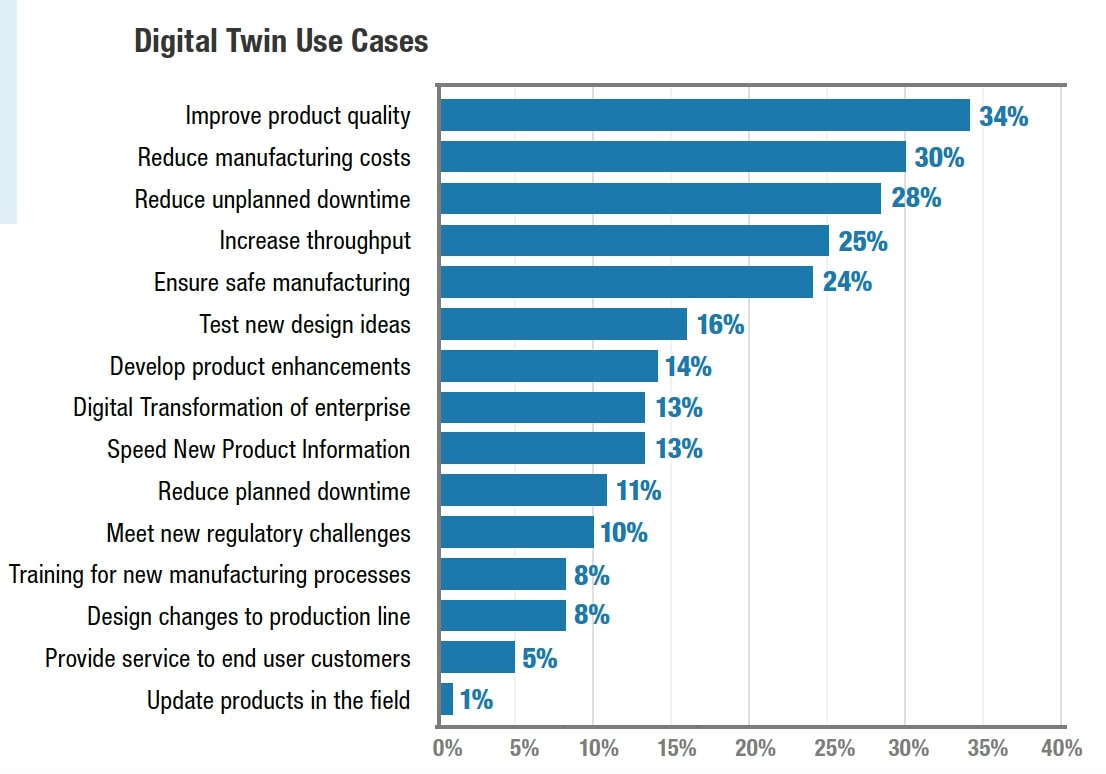
\includegraphics[scale=0.25]{6_usecases.jpg}
	\end{center}
	\caption{Pozitivni uticaji DT tehnologije\cite{usecases}}
\end{figure}

\newpage

Najveći pozitivan uticaj DT je doneo u poboljšanju kvaliteta proizvoda (+34\%),
smanjenju troškova proizvodnje (+30\%), smanjenju uskog grla u proizvodnji (+28\%), povećanje
propusnosti (+25\%) i obezbeđivanje “sigurne” proizvodnje (+24\%). \cite{values}\\

Na sledećoj slici mogu se videti četiri faze u razvijanju Digitalnog blizanca:\\
\begin{figure}[h!]
	\begin{center}
		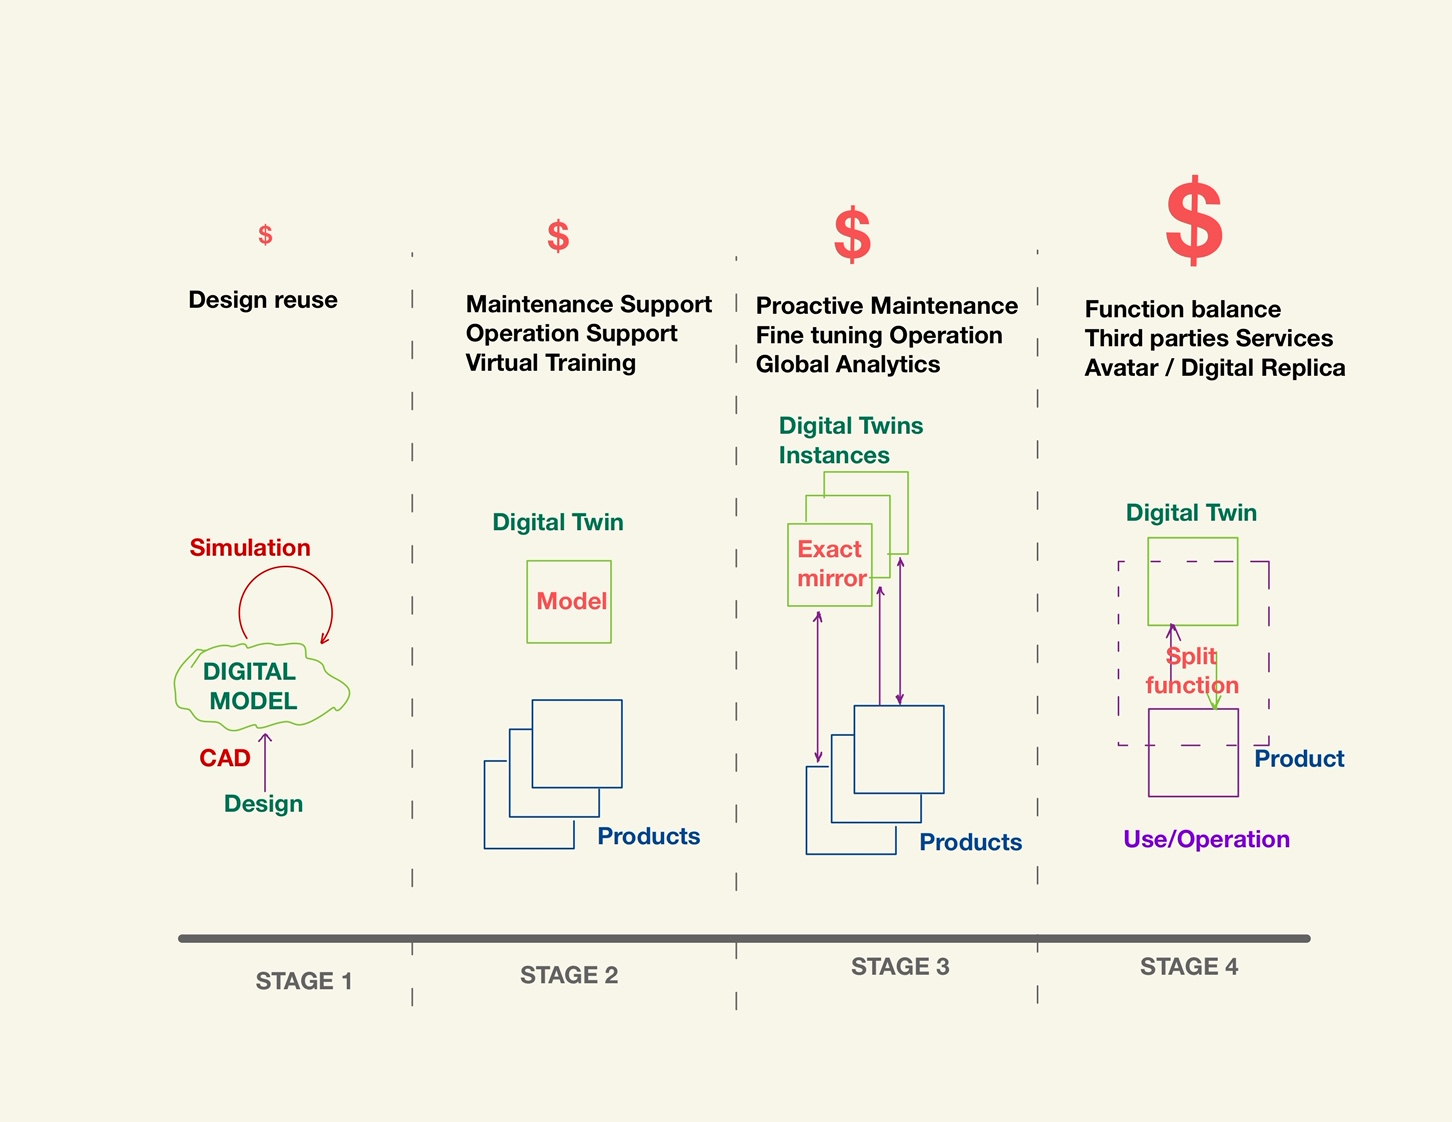
\includegraphics[scale=0.15]{7_faze_razvoja.jpg}
	\end{center}
	\caption{Faze razvoja DT\cite{economics}}
\end{figure}
\section{Primeri iz prakse}
\label{sec:primeri}

\subsection{Razvoj proizvoda}
Digitalni blizanci mogu pomoći inženjerima da testiraju izvodljivost nadolazećih proizvoda pre
lansiranja. Prema rezultatima ispitivanja, inženjeri počinju proizvoditi ili preusmeravaju fokus na
stvaranje krajnjeg proizvoda. \cite{lider}

\subsection{Prilagođavanje dizajna}
Uz pomoć digitalnih blizanaca kompanije mogu dizajnirati razne permutacije proizvoda tako da
svojim kupcima u velikoj meri mogu ponuditi personalizovane proizvode i usluge. \cite{lider}

\subsection{Automobilska i vazduhoplovna industrija}
Novi automobili uglavnom se razvijaju u virtuelnom okruženju. Blizanci se koriste u stvaranju
virtuelnog modela povezanog vozila. Simuliraju i analiziraju fazu proizvodnje i probleme koji bi
se mogli pojaviti kad vozilo izađe na put.\cite{lider}

\subsection{Razvoj automobilske industrije}
Iako se postupci digitalnih blizanaca mogu upotrebiti u tradicionalnoj automobilskoj industriji,
digitalni blizanci su zgodni i za autonomne kompanije koje se bave vozilima. Automobili koji
samostalno upravljaju sadrže mnogo senzora koji prikupljaju podatke o vozilu i okruženju
automobila. Zbog pitanja odgovornosti koja okružuju autonomna vozila, stvaranje digitalnog
blizanca automobila i testiranje svih aspekata vozila pomaže kompanijama da se osiguraju od
neočekivane štete.\cite{lider}

\subsection{Zdravstvo}
Digitalni blizanci mogu pomoći pružaocima zdravstvenih usluga da virtualizuju zdravstveno
iskustvo radi optimizacije, distribucije i troškova. Za zdravstvenu zaštitu slučajevi upotrebe mogu
se podeliti u dve grupe:
\begin{itemize}
\item poboljšanje učinkovitosti zdravstvenih operacija
\item stvaranje digitalnog blizanca bolnice, operativnih strategija, kapaciteta, osoblja i modela
distribucije.\cite{lider}
\end{itemize}

\subsection{Poboljšanje personalne nege}
Pružaoci zdravstvenih usluga i farmaceutske struke takođe se mogu koristiti digitalnim
blizancima – za modeliranje koda genoma ili fizioloških karakteristika, tako da zdravstvene
ustanove mogu pružiti personalnu negu, poput jedinstvenih lekova za svakog pacijenta. \cite{lider}

\subsection{Lanac distribucije}
Digitalni blizanci takođe se široko upotrebljavaju u lancu distribucije i logističkoj industriji.\cite{lider}

\subsection{Primena u Srbiji}
Do pojave ove tehnologije u Srbiji je prvi put došlo na leto 2020. godine. Kompanija TeamCAD
napravila je prvog digitalnog blizanca u Srbiji - istovetnu kopiju postojećeg ili projektovanog
objekta u digitalnom formatu, koja se u građevinskoj industriji koristi za izračunavanje cene
održavanja različitih komponenti, sistema, sklopova i objekata, tako što se na njihovim
replikama u digitalnom formatu rade različite simulacije pojava i procesa koje bi se dešavale i na
postojećim objektima.\cite{smartconnecting}

Digitalni blizanac napravljen je za tržni centar SAD NOVI BAZAAR u centru Novog Sada,
kojim upravlja Mat-Real Estate. Hronološki gledano, BIM model se može posmatrati kao sam
početak generisanja digitalnog blizanca, tj. kao njegova polazna tačka. Međutim, BIM model ne
može u potpunosti zadovoljiti zahteve koji se stavljaju pred model digitalnog blizanca, koji mogu
biti simulacija životnog ciklusa zgrade, različite vrste simulacije proizvodnog procesa u
industriji, simulacija ponašanja zgrade tokom požara, evakuacija ljudi tokom požara, simulacija
testova sudaranja u automobilskoj industriji, kretanje čestica i njihovo ponašanje tokom kretanja
itd. \cite{smartconnecting}

BIM 3D model je preveden iz Autodesk Revit-a sa svim informacijama, dok je ostatak aplikacije
programiran u JavaScript programskom jeziku, oslanjajući se na jQuery, Bootstrap, Node, Node
Express itd. Uz pomoć ponuđene web-aplikacije, moguće je pristupiti digitalnom blizancu iz bilo
kog modernijeg internet pretraživača, a preporuka je da to bude Google Chrome. \cite{smartconnecting}

\begin{figure}[h!]
	\begin{center}
		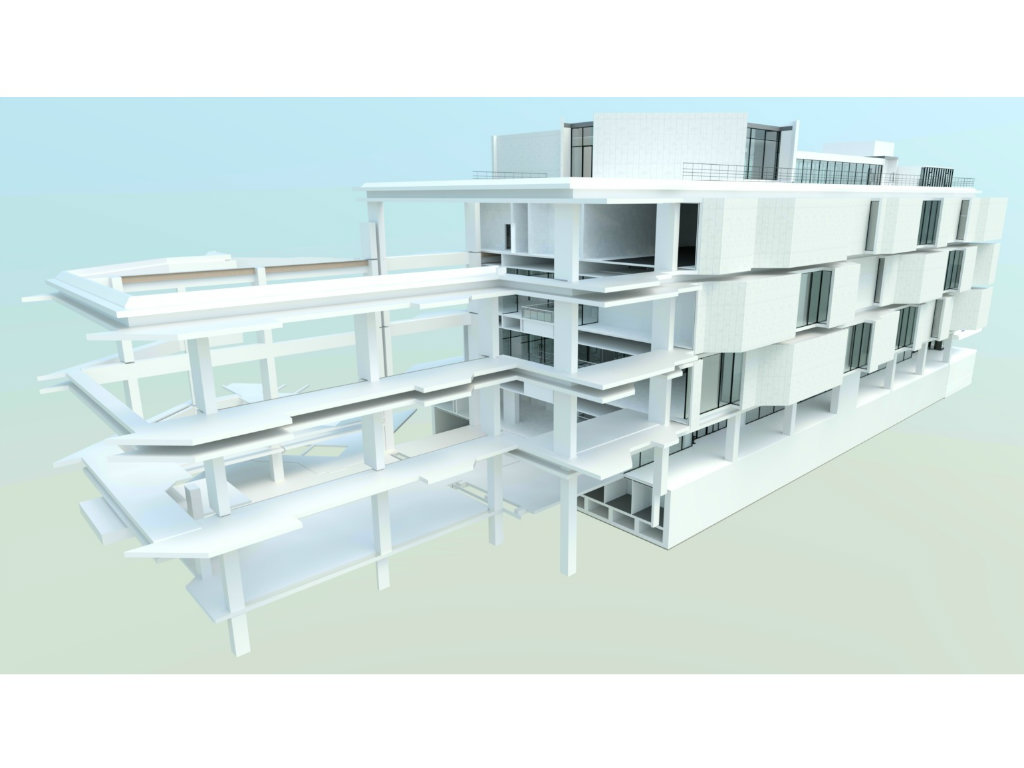
\includegraphics[scale=0.35]{8_bazaar.jpg}
	\end{center}
	\caption{Prvi Digitalni blizanac u Srbiji (projekcija) \cite{ekapija}}
\end{figure}


\section{Zaključak}
\label{sec:zakljucak}

Porast u upotrebi DT tehnologije se primećuje u poslednjih par godina, praćen rastom u
broju objavljenih istraživanja i pojačanog investiranja industrijskih lidera u razvoj ove
tehnologije. Ono što je zapravo omogućilo ovaj razvoj jeste porast u razvoju veštačke
inteligencije. \cite{enablingtechnologies}

Najšira oblast primene DT se zapaža u industriji proizvodnje. Upravo ova industrija
je najzaslužnija za razvijanje tehnologije putem učešća u istraživanjima i podelom praktičnog
znanja. Da bi se ova tehnologija iskoristila u punom potencijalu bitno je savladati prepreke poput
manjka standardizacije i netačnog definisanja DT. \cite{enablingtechnologies}

Ti standardi mogu varirati od toga kog je formata fajl za čuvanje podataka, do detalja o tome
kako se podaci mogu skladištiti, sve do zahteva o zaštiti podataka i razlika u zakonima na tu
temu širom sveta. Na kraju i samo društvo igra određenu ulogu u prihvatanju novih tehnologija.
Potrebno je da ljudi prepoznaju kada će one doneti značajne promene u našim privatnim i
profesionalnim životima. \cite{values}

\newpage

\addcontentsline{toc}{section}{Literatura}
\appendix

\iffalse
\bibliography{reference} 
\bibliographystyle{plain}
\fi

\begin{thebibliography}{9}
	
\bibitem{digitaltwins} Fei Tao, Quinglin Qi, Lihui Wang, A.Y.C. Nee. \emph{SDigital Twins and Cyber-Physical System toward Smart Manufacturing and Industry 4.0 : Correlation
	and Comparison}, 2019

\bibitem{IoT} Arquimedes Canedeo. \emph{Industrial IoT Lifecycle via Digital Twins}, 2016

\bibitem{feature} Juuso Autiosalo, Jari
Vepsalainen, Raine Viitala, Kari Tammi. \emph{A Feature – Based Framework for Structuring Industrial Digital Twins}, 2017

\bibitem{cyber} Christos Koulamas,
Athanasios Kalogeras. \emph{Cyber – Physical Systems and Digital Twins in the Industrial Internet of Things}, 2019

\bibitem{enablingtechnologies} Aidan Fuller, Zhong Fan,
Charles Day, Chris Barlow. \emph{Digital Twin: Enabling Technologies, Challenges and Open Research}, 2020

\bibitem{values} Adil Rasheed, Omer
San, Trond Kvamsdal. \emph{Digital Twin: Values, Challenges and Enablers from a Modeling Perspective}, 2020

\bibitem{ekapija} \href{https://www.ekapija.com/news/2895427/napravljen-prvi-digitalni-blizanac-u-srbiji-stedljiva-uzdanica-4-industrijske-revolucije-foto}{Prvi Digitalni blizanac u Srbiji}

\bibitem{lider}
\href{https://lidermedia.hr/tehno/digitalni-blizanci-jos-ne-idu-po-speceraj-ali-olaksavaju-poslovanje-135754}{Digitalni blizanci još ne idu po špeceraj, ali olakšavaju poslovanje}

\bibitem{smartconnecting} Porter Michael, Heppelman James. \emph{How smart, connected products are transforming companies}, 2015

\bibitem{understanding}
\href{https://www.chemengonline.com/understanding-the-digital-twin/}{Understanding The Digital Twin}

\bibitem{groundedteory}
\href{https://statswork.com/blog/what-is-grounded-theory-in-accounting-research/}{What Is Grounded Theory In Accounting Research?}

\bibitem{sticker}
\href{https://myloview.com/sticker-digital-twin-concept-icons-set-digital-twin-characteristics-no-F97B2FB}{Sticker: Digital twin concept icons set}

\bibitem{usecases}
\href{https://blogs.3ds.com/exalead/2019/07/03/digital-twin-use-cases-in-manufacturing-part-5-12/}{Digital Twin Use Cases in Manufacturing}

\bibitem{economics}
\href{URLhttps://cmte.ieee.org/futuredirections/2020/07/11/the-economics-of-the-digital-transformation-viii/}{The economics of the Digital Transformation}

\bibitem{featuredt}
\href{https://www.anylogic.com/features/digital-twin/}{Digital Twins an Example}

\bibitem{digitalinfrastructures}
Tilson David, Lyytinen Kalle, Sørensen
Carsten. \emph{Digital Infrastructures: The Missing IS Research Agenda}, 2010

\bibitem{seeingdouble}
Hamilton, Dean. \emph{Seeing double: why IoT digital twins will change the face of manufacturing}, 2018

\bibitem{sensordata}
Cai, Yi. \emph{Sensor Data and Information Fusion to Construct Digital-twins Virtual Machine Tools for Cyber-
	physical Manufacturing}, 2017

\bibitem{autonomy}
Rosen,
Roland; von Wichert, Georg; Lo, George; Bettenhausen, Kurt D. \emph{About The Importance of Autonomy and Digital Twins for the Future of Manufacturing}, 2015




\end{thebibliography}


\end{document}
